In this exercise, I empirically evaluate the performance of the UCRL2 (Jaksch et al., 2010) and UCRL2-L algorithms on a 6-state RiverSwim MDP. The main differences between the two algorithms lie in the construction of their confidence intervals. For UCRL2, the confidence sets are defined as
\[
\left| \hat{R}_t(s,a) - R' \right| \leq \sqrt{\frac{3.5\log\left(\frac{2SAn}{\delta}\right)}{n}}, \quad
\| \hat{P}_t(\cdot|s,a) - P' \|_{1} \leq \sqrt{\frac{14S\log\left(\frac{2An}{\delta}\right)}{n}},
\]
where \(n = \max(1, N_t(s,a))\). In contrast, UCRL2-L uses improved (Laplace-based) confidence intervals.

\subsection*{(i) Implementation Modifications}
To implement UCRL2, I modified the provided \texttt{UCRL2\_L.py} file. The modifications consisted of replacing the confidence set definitions used in UCRL2-L with those above. A code snippet illustrating the essential differences is as follows:

\begin{lstlisting}[language=Python]
self.confR[s, a] = sqrt((3.5 * log((2 * self.nS * self.nA * n) / self.delta)) / n)
self.confP[s, a] = sqrt((14 * self.nS * log((2 * self.nA * n) / self.delta)) / n)
\end{lstlisting}

This ensures that UCRL2 uses the appropriate theoretical confidence intervals as in Jaksch et al. (2010).

\subsection*{(ii) Cumulative Regret Evaluation}
The experiments were conducted on the 6-state RiverSwim MDP with the following settings:
\begin{itemize}
  \item Time horizon \( T = 3.5 \times 10^5 \)
  \item Initial state: left-most state (state 1)
  \item Failure probabilities: \( \delta_{\text{UCRL2}} = 0.05 \) and \( \delta_{\text{UCRL2-L}} = 0.0125 \)
\end{itemize}

The regret is defined as
\[
R(T) = \sum_{t=1}^{T} \left( g^{\star} - r_t \right),
\]
where \( g^{\star} \) is the optimal gain computed via Value Iteration.

Figure~\ref{fig:cum_regret} shows the cumulative regret curves for UCRL2 and UCRL2-L, averaged over 50 independent runs.

\begin{figure}[H]
  \centering
  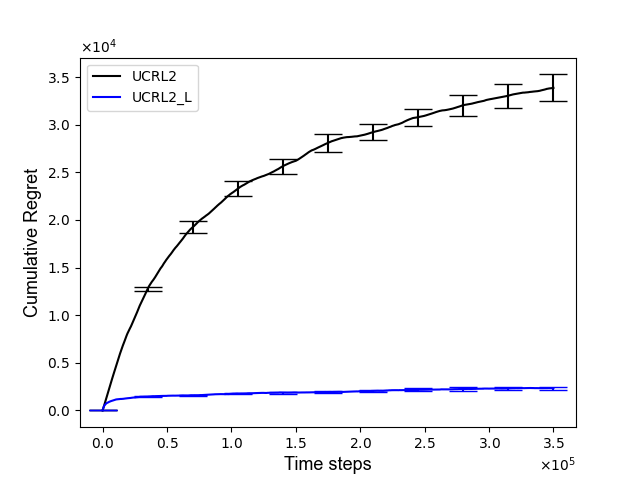
\includegraphics[width=0.8\textwidth]{Code/3/Figure_UCRL2_UCRL2_L_cumulative_regret_comparison.png}
  \caption{Average Cumulative Regret for UCRL2 and UCRL2-L over 50 runs.}
  \label{fig:cum_regret}
\end{figure}

\subsection*{(iii) Empirical Gain Comparison}
I also plotted the empirical average gain,
\[
\bar{r}(t)= \frac{1}{t}\sum_{t'=1}^{t} r_{t'},
\]
for both algorithms. In the plot, I added a horizontal dashed red line corresponding to the optimal gain \( g^{\star} \).

Figure~\ref{fig:gain} shows the gain curves along with the line for \( g^{\star} \).

\begin{figure}[H]
  \centering
  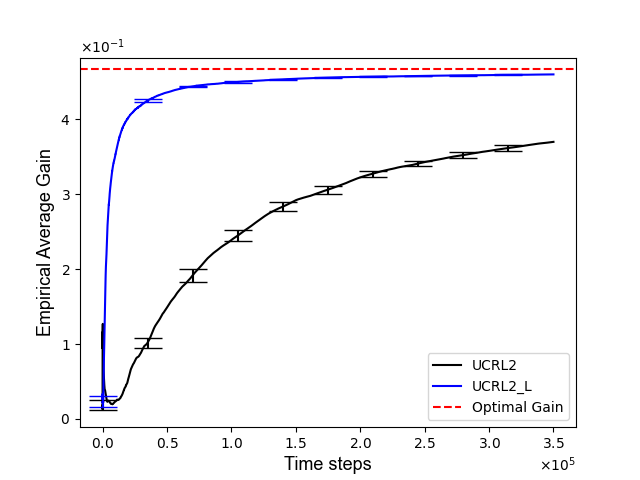
\includegraphics[width=0.8\textwidth]{Code/3/Figure_UCRL2_UCRL2_L_gain_comparison.png}
  \caption{Empirical Average Gain for UCRL2 and UCRL2-L with the optimal gain \( g^{\star} \) indicated by the horizontal red dashed line.}
  \label{fig:gain}
\end{figure}

\subsection*{(iv) Average Number of Episodes}
The average number of episodes initiated by the two algorithms across 50 runs is reported below:
\begin{itemize}
  \item UCRL2: 75.8 episodes
  \item UCRL2-L: 56.16 episodes
\end{itemize}

\subsection*{(v) Discussion}
The experimental results reveal several important differences:

\begin{enumerate}
  \item \textbf{Cumulative Regret:} The cumulative regret curve for UCRL2-L is lower than that of UCRL2, indicating that UCRL2-L achieves better performance in terms of regret minimization.
  \item \textbf{Empirical Gain:} Both algorithms approach the optimal gain \( g^{\star} \) as time progresses; however, the gain curve for UCRL2-L remains closer to \( g^{\star} \) compared to that of UCRL2. The horizontal line marking \( g^{\star} \) confirms that UCRL2-L has a smaller gap.
  \item \textbf{Number of Episodes:} UCRL2-L initiates fewer episodes on average (56.16) than UCRL2 (75.8). A smaller number of episodes is indicative of more efficient exploration and fewer policy restarts.
\end{enumerate}

Overall, the refined confidence sets in UCRL2-L appear to lead to improved empirical performance. They not only reduce the cumulative regret but also result in fewer episodes needed during learning, which suggests that UCRL2-L is more sample efficient when compared to UCRL2.

\bigskip

\noindent\textbf{Conclusion:} Based on the empirical evaluation, I conclude that UCRL2-L outperforms UCRL2 in this particular RiverSwim setting. The combination of lower cumulative regret, more stable gain curves, and fewer episodes suggests that the modifications introduced in UCRL2-L provide a practical advantage.